\documentclass{acm_proc_article-sp}
\usepackage{booktabs}
\usepackage{multicol}
\usepackage{listings}
\usepackage{algorithm}
\usepackage{algpseudocode}
\usepackage{amsmath}
\usepackage{xcolor}
\usepackage{subfigure}

\begin{document}

\title{Heat Distribution Simulation with Parallel Algorithms}

\numberofauthors{1}

\author{
\alignauthor
Jianfei Chen\\
       \affaddr{Tsinghua University}\\
       \affaddr{Beijing, China}\\
       \email{chenjf10@mails.tsinghua.edu.cn}
}

\maketitle
\section{Problem Descrption and Symbol Definition}
\subsection{Problem Descrption}

There is a room of 50 ft in height and width, at the temperature of $ROOM_TEMP$. A fire place is in the middle of the top wall of the room. It has length of 20 ft and temperature of $FIREPLACE_TEMP$. The wall is at $ROOM_TEMP$ constantly and will not be heated by the fireplace. Simulate the heat distribution when the temperature is balanced. Draw it in 5$^\circ$C temperature contours.

\subsection{Symbol List}

\begin{table}[htbp]
  \centering\caption{\label{symbols}Symbol List}
  \begin{tabular}{|p{3cm}|p{5cm}|}
  \toprule
		Item & Description\\
  \midrule
		$x$ 			& Cells in height of the room. \\
		$y$ 			& Cells in width of the room. \\
		$iter$  & Max numbers of iterations in each datum. \\
		$INC\_TIME$ & Number of different scale of data processed by the increment algorithm/\\
		$INCREMENT$      & Constant used by the increment algorithm. \\
		$P$				& Number of processes. \\
		$EPSILON$		& Terminating error.\\
		$F\_INTVAL$ & Length of each frame (in ms) while displaying the result.\\
		$T_{k,i,j}$      & The temperature of cell $(i, j)$ in $k$ th iteration. \\
  \bottomrule
  \end{tabular}
\end{table}

\section{Algorithm Design}

\subsection{Laplace Approach}

For each iteration, each cell's temperature is set to the average of its four neighbours. 

\textbf{Terminating Condition:} Keep doing the iteration until $TotalError < EPSILON$, where
\begin{align}
	TotalError = \sum_{i,j} |T_{k,i,j}-T_{k-1,i,j}|
\end{align}

The effect of $epsilon$ is shown as figure \ref{effectofepsilon}.

\begin{figure} 
  \centering 
  \subfigure[$epsilon=100$]{ 
    
\includegraphics[width=3.5cm]{epsilon100.png}} 
  \hspace{1cm} 
  \subfigure[$epsilon=10$]{ 
    
\includegraphics[width=3.5cm]{epsilon10.png}}
  \subfigure[$epsilon=1$]{ 
    
\includegraphics[width=3.5cm]{epsilon1.png}}
  \hspace{1cm} 
  \subfigure[$epsilon=0.1$]{ 
    
\includegraphics[width=3.5cm]{epsilon0_1.png}}
  \caption{Effect of $epsilon$, $x = y = 300$} 
  \label{effectofepsilon} %% label for entire figure 
\end{figure}

\subsection{The Baseline Algorithm}

The baseline algorithm is to keep doing the iteration until terminating condition meets. The time complexity is $O(xy\times iter)$, space complexity is $O(xy)$.

\subsection{Increment Algorithm}

We observed that in initial iterations, the temperature of cells that stay far from the fireplace does not change. It is waste of time calculating this. To speedup the algorithm, we can use better initial values to make the heat field converges faster. To get the initial value, we can use a smaller scale data with $x/INCREMENT$, $y/INCREMENT$ size. Since the data is small, it converges much faster than the original one. Thus, the solution of the smaller data can be used as the initial value of the original data, with scratching the temperature field of $x/INCREMENT$, $y/INCREMENT$ to $x, y$. This process can be applied multiple times, we set $INC\_TIME=8$ in this problem.

Assuming the smaller scale problem converges as slow as the original one, the time complexity has an upper bound of $xy\times iter + \frac{xy\times iter}{INCREMENT^2} + \frac{xy\times iter}{INCREMENT^4} + ... = O(xy\times iter)$. This implies the increment algorithm is not slow than the baseline algorithm in asymptotic time complexity. The space complexity is $O(xy)$, the same as the original one.

A pseudocode is shown as algorithm \ref{alg_increment}.

\begin{algorithm}                     
\caption{The increment algorithm of heat distribution problem}        
\label{alg_increment}                         
\begin{algorithmic}
	\Function{HeatDistribution}{$x$, $y$, $INC\_TIME$}
		\If {$INC\_TIME>0$}
			\State $T' \Leftarrow$ HeatDistribution($x/INCREMENT$, $y/INCREMENT$, $INC\_TIME-1$)
		\Else
			\State $T' \Leftarrow$ the initial heat field
		\EndIf
 		\For {$i = 0 \to x-1$}
 			\For {$j = 0 \to y-1$}
 				\State $T_{i,j} \Leftarrow T'_{i/INCREMENT, j/INCREMENT}$
 			\EndFor
 		\EndFor
 		\While{$T$ not converges}
 			\State Laplace-iterate($T$)
 		\EndWhile
 		\Return $T$
    \EndFunction
\end{algorithmic}
\end{algorithm}

\subsection{OpenMP Parallel Algorithm}

We make the problem parallel by processing the rows of rooms parallel. The time complexity reduces to $O(xy\times iter/P)$. We use static scheduling, thus the number of create and join operation will be $O(P\times iter)$.

\subsection{PThread Parallel Algorithm}

The pthread algorithm has nearly same implmentation as OpenMP. Excepting mutex has been used to wake up and wait for threads. The number of create and join operation has been reduced to $O(P)$, while the time and space complexity remains the same as OpenMP, i.e., $O(xy\times iter/P)$ and $O(xy)$.

\subsection{MPI Parallel Algorithm}

We divide the room into blocks for the subprocesses to compute. Blocks scheme is better because it have lower communication overhead comparing with strip scheme.

\begin{align}
	StripOverhead = 2max\{x,y\}P\\
	BlockOverhead = 4max\{x,y\}P^{0.5}
\end{align}

Apparently, $StripOverhead > BlockOverhead$ when $P>4$. A MPI pseudocode is as algorithm \ref{alg_mpi_increment}.

\begin{algorithm}                     
\caption{The MPI increment algorithm of heat distribution problem}        
\label{alg_mpi_increment}                         
\begin{algorithmic}
	\Function{HeatDistribution}{$x$, $y$, $INC\_TIME$}
		\If{$INCREMENT\_TIME>0$}
			\State $T' \Leftarrow$ HeatDistribution($x/INCREMENT$, $y/INCREMENT$, $INCREMENT\_TIME-1$)
		\Else
			\State $T' \Leftarrow$ the initial heat field
		\EndIf
		\For {$i = 0 \to x-1$}
			\For {$j = 0 \to y-1$}
				\State $T_{i,j} \Leftarrow T'_{i/INCREMENT, j/INCREMENT}$
			\EndFor
		\EndFor
		\State scatter $T$ to subprocesses
		\While{$T$ not converges}
			\State Laplace-iterate($T$)
		\EndWhile
		\State gather $T$ from subprocesses
		\Return $T$
    \EndFunction
    
    \Function{Laplace-iterate}{$T$}
		\State send topmost, bottommost row and leftmost, rightmost columns to neighbours
		\State receive topmost, bottommost row and leftmost, rightmost columns from neighbours
		\State $T'' \Leftarrow T$
		\For {$i = 0 \to x/P^{0.5}-1$}
			\For {$j = 0 \to y/P^{0.5}-1$}
				\State $T_{i,j} \Leftarrow (T''_{i-1,j}+T''{i+1,j}+T''{i,j-1}+T''{i,j+1})/4$
			\EndFor
		\EndFor	
		\Return $T$
    \EndFunction
\end{algorithmic}
\end{algorithm}

The time complexity is $O(xy\times iter/P)$, space complexity is $O(xy)$, communication overhead is $O(max\{x,y\}P^{0.5}\times iter+xy\times INC\_TIME)$, approximately $O(max\{x,y\}P^{0.5}\times iter)$.

\subsection{Summary}

The complexity of mentioned algorithms is summarized as table \ref{timecomplexity}.

\begin{table}[htbp]
  \centering\caption{\label{timecomplexity}Complexity of heat simulation algorithm}
  \begin{tabular}{cc}
  \toprule
		\textbf{Algorithm} & \textbf{Time(computation)} \\
  \midrule
		Baseline & $O(xy\times iter)$ \\
		Increment & $O(xy\times iter)$ \\
		OpenMP\_Increment & $O(xy\times iter/P)$ \\
		PThread\_Increment & $O(xy\times iter/P)$ \\
		MPI\_Increment & $O(xy\times iter)$ \\
   \midrule
   \textbf{Algorithm} & \textbf{Time(overhead)}\\
   \midrule
		Baseline & $O(xy)$ \\
		Increment & $O(xy)$ \\
		OpenMP\_Increment & $O(xy)$ \\
		PThread\_Increment & $O(xy)$ \\
		MPI\_Increment & $O(xy)$ \\
   \midrule
   \textbf{Algorithm} & \textbf{Space}\\
   \midrule
		Baseline & $O(xy\times iter)$ \\
		Increment & $O(xy\times iter)$ \\
		OpenMP\_Increment & $O(xy\times iter/P)$ \\
		PThread\_Increment & $O(xy\times iter/P)$ \\
		MPI\_Increment & $O(xy\times iter)$ \\ 
  \bottomrule
  \end{tabular}
\end{table}

\section{Experimental Methology}
The experiment is done on a dual chip computer with 12 cores at 2.93GHz and an cluster with 20 nodes respectively. 
\begin{table}[htbp]
  \centering\caption{\label{MPI}Experiment Configurations}
  \begin{tabular}{|p{3cm}|p{4cm}|}
  \hline
  System Configurations1 & Intel Xeon X5670x2, 6 Cores \@ 2.93GHz, 12MB Cache\\
  \hline
  System Configurations2 & 20 nodes, each nodes is Intel Xeon X5670x2, 6 Cores \@ 2.93GHz, 12MB Cache\\
  \hline
  Compiler (PThread\&OpenMP) & gcc \\
  \hline
  Compiler (MPI) & Intel C Compiler\\
  \hline
  MPI & Intel MPI\\
  \hline
  PThread & PThread \\
  \hline
  OpenMP & OpenMP\\
  \hline
  \end{tabular}
\end{table}

The parameters of base test data is as table \ref{basetestdata}, all the experiment parameters are modified from the beast test data.
\begin{table}[htbp]
  \centering\caption{\label{MPI}Experiment Configurations}
  \begin{tabular}{|c|c|}
  \hline
  Parameter & Value \\
  \hline
  $x$	& 300 \\
  \hline
  $y$   & 300 \\
  \hline
  $iter$ & $1000000$(until converges) \\
  \hline
  $epsilon$ & 1 \\
  \hline
  $INC\_TIME$ & 8\\
  \hline
  $INCREMENT$ & 1.6\\
  \hline
  \end{tabular}
\end{table}

\section{Experimental Results}

\subsection{Baseline}

The performance of the baseline algorithm on base test data is as table \ref{baseline}.

\begin{table}[htbp]
  \centering\caption{\label{baseline}Baseline Algorithm Performance}
  \begin{tabular}{|c|c|}
  \hline
  iterations & time/s \\
  \hline
  67125 & 120.132760\\
  \hline
  \end{tabular}
\end{table}

\subsection{Speedup of the Increment Algorithm}
\subsubsection{Impact of the scale factor $INCREMENT$}
We run the base test data and tried different scale factors, from 1.3 to 1.9. The total number of iterations and time consumption is as figure \ref{impactscalefactor}. We can observe that both number of iterations and time consumption reached minimum at $INCREMENT=1.6$.

\begin{figure}[htbp]
\centering 
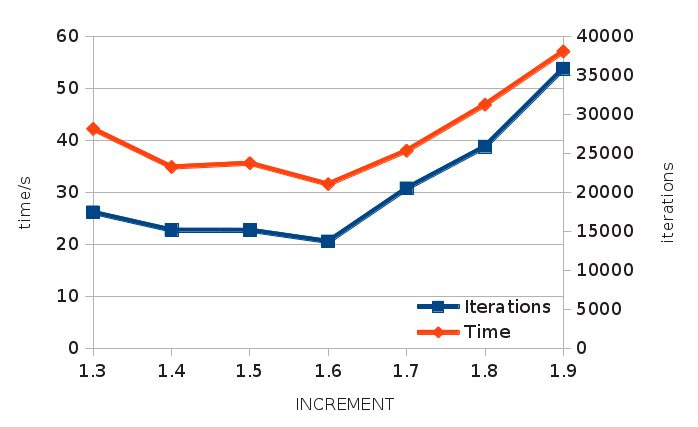
\includegraphics[width=7.5cm]{impactscalefactor.png}
\caption{Impact of the scale factor $INCREMENT$}
\label{impactscalefactor} 
\end{figure}

\subsubsection{Impact of problem scale}

To make the parameter selection more convincing, we calculate $INCREMENT$ at different scale, as table \ref{TIncrementScale}. 

\begin{table}[htbp]
  \centering\caption{\label{TIncrementScale}Optimal $INCREMENT$ at different scale}
  \begin{tabular}{|c|c|c|c|c|}
  \hline
  $x, y$ & 200 & 250 & 300 & 350\\
  \hline
  Optimal $INCREMENT$ & 1.6 & 1.4 & 1.6 & 1.4\\
  \hline
  \end{tabular}
\end{table}

The time consumption at different scale and $INCREMENT$ is as figure \ref{differentscaledifferentfactortime}. About 6x speedup is achieved at the base test data.

\begin{figure}[htbp]
\centering 
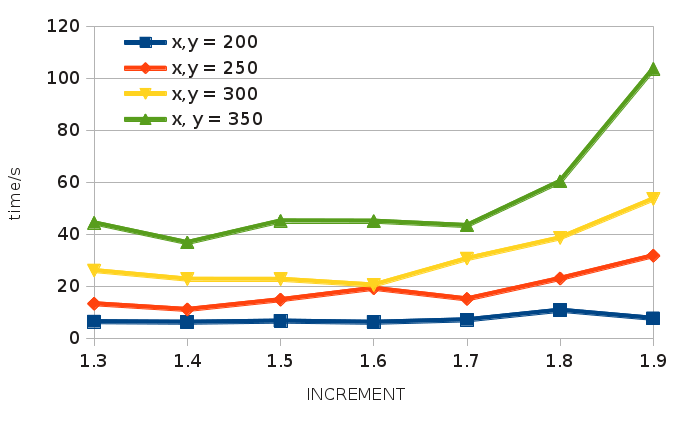
\includegraphics[width=7.5cm]{differentscaledifferentfactortime.png}
\caption{Time consumption of baseline and increment algorithm with different scale and $INCREMENT$}
\label{differentscaledifferentfactortime} 
\end{figure}

The time consumption and speedup of baseline and increment algorithm at different scale is shown as figure \ref{scaleIncrementTimeConsumption}, \ref{scaleIncrementSpeedup}. 
At larger scale, the scaling up will be more precise, but $epsilon$ for each cell is more strict. So the speedup increase with fluctuation.

\begin{figure}[htbp]
\centering 
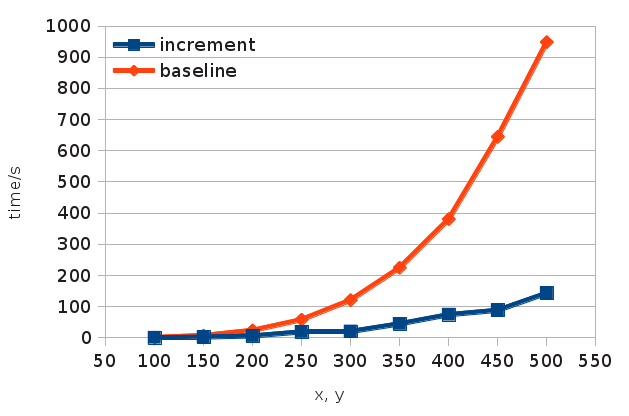
\includegraphics[width=7.5cm]{scaleIncrementTimeConsumption.png}
\caption{Time consumption of baseline and increment algorithm as scale increase}
\label{scaleIncrementTimeConsumption} 
\end{figure}

\begin{figure}[htbp]
\centering 
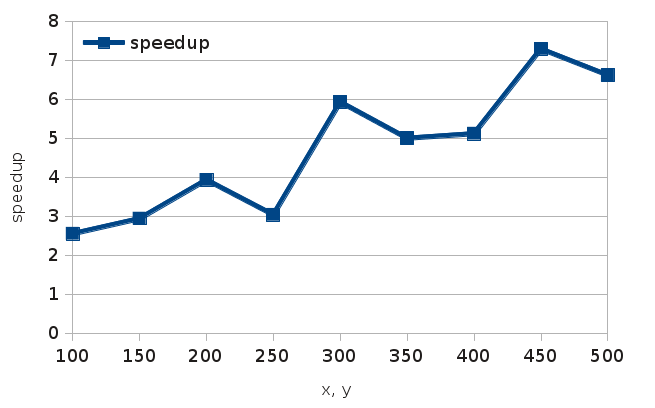
\includegraphics[width=7.5cm]{scaleIncrementSpeedup.png}
\caption{Speedup of baseline and increment algorithm as scale increase}
\label{scaleIncrementSpeedup} 
\end{figure}

\subsubsection{Impact of $epsilon$}

To make the parameter selection more convincing, we calculate $INCREMENT$ at different $epsilon$, as table \ref{TEpsilonScale}.

\begin{table}[htbp]
  \centering\caption{\label{TEpsilonScale}Optimal $INCREMENT$ at different $epsilon$}
  \begin{tabular}{|c|c|c|c|}
  \hline
  $Epsilon$ & 1 & 0.1 & 0.01\\
  \hline
  Optimal $INCREMENT$ & 1.6 & 1.6 & 1.6\\
  \hline
  \end{tabular}
\end{table}

The time consumption at different $epsilon$ and $INCREMENT$ is as figure \ref{differentepsilondifferentfactortime}.

\begin{figure}[htbp]
\centering 
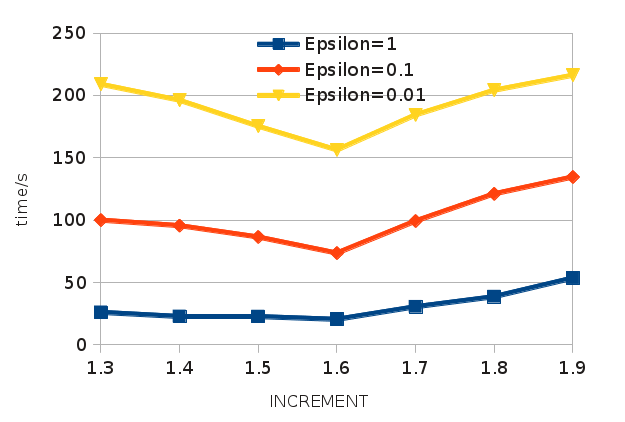
\includegraphics[width=7.5cm]{differentepsilondifferentfactortime.png}
\caption{Time consumption of baseline and increment algorithm with different $epsilon$ and $INCREMENT$}
\label{differentepsilondifferentfactortime} 
\end{figure}

The time consumption and speedup of baseline and increment algorithm at different $epsilon$ is shown as figure \ref{epsilonIncrementTimeConsumption}, \ref{epsilonIncrementSpeedup}. 
The scaling up brings intrinsic error, relatively fixed. If $epsilon$ scales down, the speedup converging from the initial state to the intrinsic error state will be outnumber by that computing from the intrinsic error state to $epsilon$ error state. So the speedup is converging to 1. However, since we proved that $epsilon=1$ is enough, the effect can be neglected. 

\begin{figure}[htbp]
\centering 
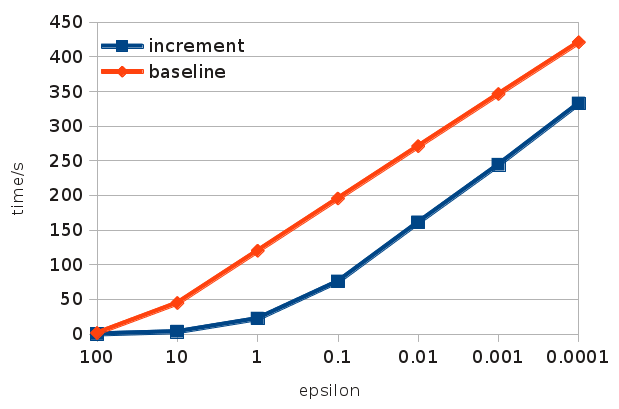
\includegraphics[width=7.5cm]{epsilonIncrementTimeConsumption.png}
\caption{Time consumption of baseline and increment algorithm as $epsilon$ decrease}
\label{epsilonIncrementTimeConsumption} 
\end{figure}

\begin{figure}[htbp]
\centering 
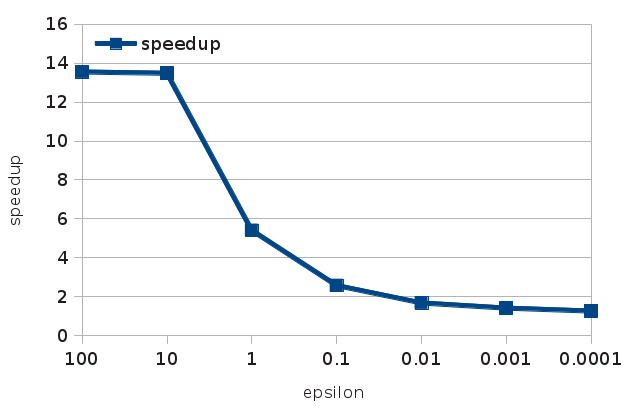
\includegraphics[width=7.5cm]{epsilonIncrementSpeedup.png}
\caption{Speedup of baseline and increment algorithm as $epsilon$ decrease}
\label{epsilonIncrementSpeedup} 
\end{figure}

\subsection{Parallel Algorithm Speedup}

The parallel algorithm time consumption and speedup on machine 1 is shown as figure \ref{parallelalgtime}, \ref{parallelalgspeedup}. About 60x speedup is achieved by OpenMP with 12 cores.

\begin{figure}[htbp]
\centering 
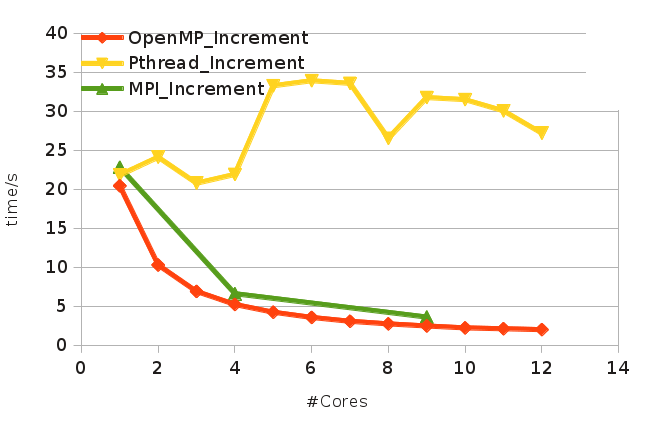
\includegraphics[width=7.5cm]{parallelalgtime.png}
\caption{Time consumption of parallel algorithm}
\label{parallelalgtime} 
\end{figure}

\begin{figure}[htbp]
\centering 
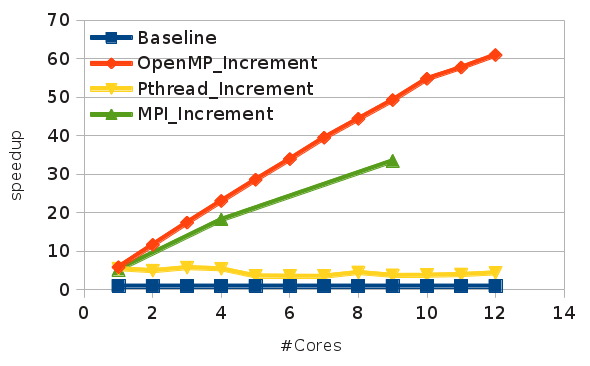
\includegraphics[width=7.5cm]{parallelalgspeedup.png}
\caption{Speedup of parallel algorithm}
\label{parallelalgspeedup} 
\end{figure}

\section{Conclusion}

By appling the increment algorithm and OpenMP, up to 60x of increment is achieved. MPI on clusters can provide further speedup.

\section{Experience}
\begin{enumerate}
	\item On memory intensive applicantions, parallel algorithm may not provide speedup.
	\item Replacing create and join with mutexs wake up and wait may cause the program faster.
\end{enumerate}

\section{Appendix A: Instruction for using the experiment programs}

Compiler Options: 

\textbf{DISPLAY}: Create output.

Compile:

\textbf{make all}: Make all programs, without display.

\textbf{make -f Makefile\_Display all}: Make all programs, with display.

Command Line Parameters:

\textbf{PThread\&OpenMP:} ./temperature\_openxy/pthread $x$, $y$, $iter$, $INC_TIME$, $INCREMENT$, $P$, $epsilon$

\textbf{MPI:} mpirun -n $P$ ./temperature\_mpi $x$, $y$, $iter$, $INC\_TIME$, $INCREMENT$, $epsilon$

\section{Appendix B: Programs}

\begin{lstlisting}[caption=const.h]
#ifndef _CONST
#define _CONST

#define FRAME_INTERVAL 20
#define X_REFRESH_RATE 1000

#define ROOM_TEMP 20
#define FIRE_TEMP 100

#endif
\end{lstlisting}

\begin{lstlisting}[caption=models.h]
#ifndef _MODELS
#define _MODELS

#include <memory.h>
#include <stdlib.h>
#include "const.h"

#define legal(x, n) ( (x)>=0 && (x)<(n) )

typedef struct TemperatureField
{
	int x, y;
	double **t;
	double *storage;
}TemperatureField;

void deleteField(TemperatureField *field);

void newField(TemperatureField *field, int x, int y, int sourceX, int sourceY)
{
	TemperatureField temp = *field;
	field->storage = malloc( sizeof(double) * x * y );
	field->t = malloc( sizeof(double*) * x );
	field->x = x;
	field->y = y;
	int i, j;
	for (i=0; i<x; ++i)
		field->t[i] = &field->storage[i*y];
	if (sourceX)
	{
		double scaleFactorX = (double)sourceX/x;
		double scaleFactorY = (double)sourceY/y;
		for (i=0; i<x; ++i)
			for (j=0; j<y; ++j)
				field->t[i][j] = temp.t[(int)(i*scaleFactorX)][(int)(j*scaleFactorY)];
		deleteField(&temp);
	}
	else memset(field->storage, 0, sizeof(double)*x*y);
}

void initField(TemperatureField *field)
{
	int i, j;
	for (i=0; i<field->x; ++i)
		for (j=0; j<field->y; ++j)
			field->t[i][j] = 20.0f;
}

void refreshField(TemperatureField *field, int initX, int initY, int thisX, int thisY, int allX, int allY)
{
	int j;
	for (j=allY*3/10; j<allY*7/10; ++j)
	    if (legal(-initX, thisX)&&legal(j-initY, thisY))
		field->t[-initX][j-initY] = 100.0f;
}

TemperatureField* myClone(TemperatureField *field, int X, int Y)
{
	int i, j;
        TemperatureField *ret = malloc(sizeof(TemperatureField));
	ret->x = X;
	ret->y = Y;
	ret->storage = malloc(sizeof(double)*ret->x*ret->y);
	ret->t = malloc(sizeof(double*)*ret->x);
	for (i=0; i<ret->x; ++i)
		ret->t[i] = &ret->storage[i*ret->y];
	for (i=0; i<X; ++i)
		for (j=0; j<Y; ++j)
			ret->t[i][j] = field->t[i][j];
	return ret;
}

void deleteField(TemperatureField *field)
{
	free(field->t);
	free(field->storage);
	//free(field);
}

#endif

\end{lstlisting}

\begin{lstlisting}[caption=display.h]
/* Initial Mandelbrot program */


#include <X11/Xlib.h>
#include <X11/Xutil.h>
#include <X11/Xos.h>
#include <stdio.h>
#include <string.h>
#include <math.h>
#include <stdlib.h>
#include "models.h"
#include "const.h"

Window          win;                            /* initialization for a window */
unsigned
int             width, height,                  /* window size */
		border_width,                   /*border width in pixels */
		idth, display_height,  /* size of screen */
		screen;                         /* which screen */

char            *window_name = "Temperature Simulation", *display_name = NULL;
GC              gc;
unsigned
long            valuemask = 0;
XGCValues       values;
Display         *display;
XSizeHints      size_hints;
Pixmap          bitmap;
FILE            *fp, *fopen ();	
Colormap	default_cmap;
XColor		color[256];

int temperatue_to_color_pixel(double t)
{
	return color[(int)(t/5.0f)].pixel;
}

void XWindow_Init(TemperatureField *field)
{    
        XSetWindowAttributes attr[1];       
       
        /* connect to Xserver */

        if (  (display = XOpenDisplay (display_name)) == NULL ) {
           fprintf (stderr, "drawon: cannot connect to X server %s\n",
                                XDisplayName (display_name) );
        exit (-1);
        }
        
        /* get screen size */

        screen = DefaultScreen (display);

        /* set window size *///XFlush (display);

        width = field->y;
	height = field->x;

        /* create opaque window */

        border_width = 4;
        win = XCreateSimpleWindow (display, RootWindow (display, screen),
                                width, height, width, height, border_width, 
                                BlackPixel (display, screen), WhitePixel (display, screen));

        size_hints.flags = USPosition|USSize;
        size_hints.x = 0;
        size_hints.y = 0;
        size_hints.width = width;
        size_hints.height = height;
        size_hints.min_width = 300;
        size_hints.min_height = 300;
        
        XSetNormalHints (display, win, &size_hints);
        XStoreName(display, win, window_name);

        /* create graphics context */

        gc = XCreateGC (display, win, valuemask, &values);

	default_cmap = DefaultColormap(display, screen);
        XSetBackground (display, gc, WhitePixel (display, screen));
        XSetForeground (display, gc, BlackPixel (display, screen));
        XSetLineAttributes (display, gc, 1, LineSolid, CapRound, JoinRound);

        attr[0].backing_store = Always;
        attr[0].backing_planes = 1;
        attr[0].backing_pixel = BlackPixel(display, screen);

        XChangeWindowAttributes(display, win, CWBackingStore | CWBackingPlanes | CWBackingPixel, attr);

        XMapWindow (display, win);
        XSync(display, 0); 

	/* create color */
	int i;
	for (i=0; i<20; ++i)
	{
	    color[i].green = rand()%65535;
	    color[i].red = rand()%65535;
	    color[i].blue = rand()%65535;
	    color[i].flags = DoRed | DoGreen | DoBlue;
	    XAllocColor(display, default_cmap, &color[i]);
	}
}

void XResize(TemperatureField *field)
{
    XResizeWindow(display, win, field->y, field->x);
}

void XRedraw(TemperatureField *field)
{
    int i, j;
    for (i=0; i<field->x; ++i)
        for (j=0; j<field->y; ++j)
	{
		XSetForeground(display, gc, temperatue_to_color_pixel(field->t[i][j]));
	        XDrawPoint (display, win, gc, j, i);
	}
    XFlush (display);
}


\end{lstlisting}

\begin{lstlisting}[caption=main\_openmp\_increment.h]
#include "const.h"
#include "models.h"
#include "display.h"
#include <omp.h>

#define legal(x, n) ( (x)>=0 && (x)<(n) )
#define start_time clock_gettime(CLOCK_MONOTONIC, &start);
#define end_time clock_gettime(CLOCK_MONOTONIC, &finish); 
#define time_elapsed_ns (long long)(finish.tv_sec-start.tv_sec)*1000000000 + finish.tv_nsec - start.tv_nsec
#define time_elapsed_s (double)(finish.tv_sec-start.tv_sec) + (double)(finish.tv_nsec - start.tv_nsec)/1000000000
#define NOT_FIRE_PLACE i

int iteration, threads;
int INCREMENT_TIME;
double EPSILON;
double INCREMENT;
TemperatureField *field;
TemperatureField *tempField, *swapField;

int dx[4] = {0, -1, 0, 1};
int dy[4] = {1, 0, -1, 0};

int x, y, iter_cnt;

double temperature_iterate(TemperatureField *field)
{
	++iter_cnt;
	refreshField(field, 0, 0, field->x, field->y, field->x, field->y);
	int i, j, d;
	double ret = 0;
#pragma omp parallel for schedule(static) private(j) private(d) reduction(+:ret)
	for (i=0; i<field->x; ++i){
		for (j=0; j<field->y; ++j)
		{
			tempField->t[i][j] = 0;
			for (d=0; d<4; ++d)
				if ( legal(i+dx[d], field->x) && legal(j+dy[d], field->y) )
					tempField->t[i][j] += field->t[i+dx[d]][j+dy[d]];
				else
					tempField->t[i][j] += ROOM_TEMP;
			tempField->t[i][j] /= 4;
			if (NOT_FIRE_PLACE)
				ret += fabs(tempField->t[i][j] - field->t[i][j]);
		}
	}
	return ret;
}

int main(int argc, char **argv)
{
    struct timespec start, finish;
    start_time 
    if (argc<8)
    {
	    printf("Usage: %s x y iteration INCREMENT_TIME, INCREMENT threads EPSILON\n", argv[0]);
    }
    sscanf(argv[1], "%d", &x);
    sscanf(argv[2], "%d", &y);
    sscanf(argv[3], "%d", &iteration);
    sscanf(argv[4], "%d", &INCREMENT_TIME);
    sscanf(argv[5], "%lf", &INCREMENT);
    sscanf(argv[6], "%d", &threads);
    sscanf(argv[7], "%lf", &EPSILON);
    omp_set_num_threads(threads);

    field = malloc(sizeof(TemperatureField));
    tempField = malloc(sizeof(TemperatureField));
    field->x = y;
    field->y = x;
#ifdef DISPLAY
    XWindow_Init(field);
#endif

    int iter, inc;
    int *X_Size = malloc(sizeof(int)*INCREMENT_TIME);
    int *Y_Size = malloc(sizeof(int)*INCREMENT_TIME);
    X_Size[INCREMENT_TIME-1] = x;
    Y_Size[INCREMENT_TIME-1] = y;
    for (inc=INCREMENT_TIME-2; inc>=0; --inc)
    {
	X_Size[inc] = X_Size[inc+1] / INCREMENT;
	Y_Size[inc] = Y_Size[inc+1] / INCREMENT;
    }

    for (inc=0; inc<INCREMENT_TIME; ++inc)
    {	
	if (!inc)
	{
            newField(field, X_Size[inc], Y_Size[inc], 0, 0);
	    newField(tempField, X_Size[inc], Y_Size[inc], 0, 0);	    
	    initField(field);
	}
	else 
	{
            newField(field, X_Size[inc], Y_Size[inc], X_Size[inc-1], Y_Size[inc-1]);
	    newField(tempField, X_Size[inc], Y_Size[inc], X_Size[inc-1], Y_Size[inc-1]);
	}
#ifdef DISPLAY
        XResize(field);
#endif
	for (iter=0; iter<iteration; iter++)
        {
	   double error = temperature_iterate(field);
	   if (error<EPSILON)
	   {
		   printf("Finished. iteration=%d, error=%lf\n", iter, error);

		break;
	   }
	   swapField = field;
	   field = tempField;
	   tempField = swapField;
#ifdef DISPLAY
	   end_time
	   if (time_elapsed_ns > FRAME_INTERVAL*1000000)
	   {
		start_time;
		XRedraw(field);
	   } 	   
//	    	   puts("Field:");
//		   int i, j;
//        	    for (i=0; i<field->x; ++i)
//        	    {
//        		    for (j=0; j<field->y; ++j)
//        		    	printf("%lf ", field->t[i][j]);
//        		    puts("");
//        	    }
#endif	
	}
    }
    deleteField(field);
    deleteField(tempField);
    free(X_Size);
    free(Y_Size);
    printf("Finished in %d iterations.\n", iter_cnt);
    end_time;
    printf("%lf\n", time_elapsed_s);
    return 0;
}

\end{lstlisting}

\begin{lstlisting}[caption=main\_pthread\_increment.h]
#include "const.h"
#include "models.h"
#include "display.h"
#include <pthread.h>
#include <stdio.h>

#define legal(x, n) ( (x)>=0 && (x)<(n) )
#define start_time clock_gettime(CLOCK_MONOTONIC, &start);
#define end_time clock_gettime(CLOCK_MONOTONIC, &finish); 
#define time_elapsed_ns (long long)(finish.tv_sec-start.tv_sec)*1000000000 + finish.tv_nsec - start.tv_nsec
#define time_elapsed_s (double)(finish.tv_sec-start.tv_sec) + (double)(finish.tv_nsec - start.tv_nsec)/1000000000
#define NOT_FIRE_PLACE i

#define update(dx, dy) if ( legal(i+dx, field->x) && legal(j+dy, field->y) ) tempField->t[i][j] += field->t[i+dx][j+dy]; else tempField->t[i][j] += ROOM_TEMP;

int iteration, threads;
TemperatureField *field;
TemperatureField *tempField, *swapField;
pthread_t *threadPool;
pthread_mutex_t *subThreadWakeUp, *subThreadFinished;
int *threadID, terminate;
double *error;
int INCREMENT_TIME;
double INCREMENT, EPSILON;

int dx[4] = {0, -1, 0, 1};
int dy[4] = {1, 0, -1, 0};

int x, y, iter_cnt;

int min(int x, int y){ if (x<y) return x; return y; }

void* iterateLine(void* data)
{   
    int threadID = *((int*)data);
    while (1)
    {
	    pthread_mutex_lock(&subThreadWakeUp[threadID]);
	    if (terminate) break;
	    int blockSize = field->x/threads + !!(field->x%threads);
	    int lineStart = blockSize*threadID;
	    int lineEnd = min(blockSize*(threadID+1), field->x);
	    error[threadID]=0;

	    int i, j, d;
	    for (i=lineStart; i<lineEnd; ++i) 
		for (j=0; j<field->y; ++j)
		{
			tempField->t[i][j] = 0;
			for (d=0; d<4; ++d)
				if ( legal(i+dx[d], field->x) && legal(j+dy[d], field->y) )
					tempField->t[i][j] += field->t[i+dx[d]][j+dy[d]];
				else
					tempField->t[i][j] += ROOM_TEMP;
			tempField->t[i][j] /= 4;
			if (NOT_FIRE_PLACE)
				error[threadID] += fabs(tempField->t[i][j] - field->t[i][j]);
		}
	    pthread_mutex_unlock(&subThreadFinished[threadID]);
    }
    pthread_exit(NULL);
}

double temperature_iterate()
{
	++iter_cnt;
	refreshField(field, 0, 0, field->x, field->y, field->x, field->y);
	int i;

	for (i=0; i<threads; ++i)
		pthread_mutex_unlock(&subThreadWakeUp[i]);
	for (i=0; i<threads; ++i)
		pthread_mutex_lock(&subThreadFinished[i]);
	double sumError = 0;
	for (i=0; i<threads; ++i)
		sumError += error[i];

	return sumError;
}

int main(int argc, char **argv)
{
    struct timespec start, finish;
    start_time
    if (argc<8)
    {
	    printf("Usage: %s x y iteration INCREMENT_TIME, INCREMENT threads EPSILON\n", argv[0]);
    }
    sscanf(argv[1], "%d", &x);
    sscanf(argv[2], "%d", &y);
    sscanf(argv[3], "%d", &iteration);
    sscanf(argv[4], "%d", &INCREMENT_TIME);
    sscanf(argv[5], "%lf", &INCREMENT);
    sscanf(argv[6], "%d", &threads);
    sscanf(argv[7], "%lf", &EPSILON);

    field = malloc(sizeof(TemperatureField));
    tempField = malloc(sizeof(TemperatureField));
    threadPool = malloc(sizeof(pthread_t)*threads);
    subThreadWakeUp = malloc(sizeof(pthread_mutex_t)*threads);
    subThreadFinished = malloc(sizeof(pthread_mutex_t)*threads);
    threadID = malloc(sizeof(int)*threads);
    error = malloc(sizeof(double)*threads);
    terminate = 0;
    field->x = y;
    field->y = x;
#ifdef DISPLAY
    XWindow_Init(field);
#endif

    int i;
    for (i=0; i<threads; ++i)
    {
	pthread_mutex_init(&subThreadWakeUp[i], NULL);
	pthread_mutex_init(&subThreadFinished[i], NULL);
	pthread_mutex_lock(&subThreadWakeUp[i]);
	pthread_mutex_lock(&subThreadFinished[i]);
	threadID[i] = i;
	pthread_create(&threadPool[i], NULL, iterateLine, &threadID[i]);
    }

    int iter, inc;
    int *X_Size = malloc(sizeof(int)*INCREMENT_TIME);
    int *Y_Size = malloc(sizeof(int)*INCREMENT_TIME);
    X_Size[INCREMENT_TIME-1] = x;
    Y_Size[INCREMENT_TIME-1] = y;
    for (inc=INCREMENT_TIME-2; inc>=0; --inc)
    {
	X_Size[inc] = X_Size[inc+1] / INCREMENT;
	Y_Size[inc] = Y_Size[inc+1] / INCREMENT;
    }

    for (inc=0; inc<INCREMENT_TIME; ++inc)
    {	
	if (!inc)
	{
            newField(field, X_Size[inc], Y_Size[inc], 0, 0);
	    newField(tempField, X_Size[inc], Y_Size[inc], 0, 0);	    
	    initField(field);
	}
	else 
	{
            newField(field, X_Size[inc], Y_Size[inc], X_Size[inc-1], Y_Size[inc-1]);
	    newField(tempField, X_Size[inc], Y_Size[inc], X_Size[inc-1], Y_Size[inc-1]);
	}
#ifdef DISPLAY
        XResize(field);
#endif
	for (iter=0; iter<iteration; iter++)
        {	
	   double error = temperature_iterate();
	   if (error<EPSILON){
		   printf("Finished. iteration=%d, error=%lf\n", iter, error);
		break;
	   }
	   swapField = field;
	   field = tempField;
	   tempField = swapField;
#ifdef DISPLAY
	   end_time
	   if (time_elapsed_ns > FRAME_INTERVAL*1000000)
	   {
		start_time;
		XRedraw(field);
	   }
#endif	
	}
    }
#ifdef DISPLAY
    XRedraw(field);
    usleep(10000000);
#endif
    deleteField(field);
    deleteField(tempField);
    free(X_Size);
    free(Y_Size);
    free(threadPool);
    for (i=0; i<threads; ++i)
    {
	    terminate = 1;
	    pthread_mutex_unlock(&subThreadWakeUp[i]);
    }
    printf("Finished in %d iterations.\n", iter_cnt);
    end_time;
    printf("%lf\n", time_elapsed_s);
    pthread_exit(NULL);
    return 0;
}

\end{lstlisting}

\begin{lstlisting}[caption=main\_mpi\_increment.h]
#include "const.h"
#include "models.h"
#include "display.h"
#include <mpi.h>
#include <math.h>
#include <assert.h>

#define start_time clock_gettime(CLOCK_MONOTONIC, &start);
#define end_time clock_gettime(CLOCK_MONOTONIC, &finish); 
#define time_elapsed_ns (long long)(finish.tv_sec-start.tv_sec)*1000000000 + finish.tv_nsec - start.tv_nsec
#define time_elapsed_s (double)(finish.tv_sec-start.tv_sec) + (double)(finish.tv_nsec - start.tv_nsec)/1000000000
#define fillReceiveBuffer for (i=0; i<line_buffer_size; ++i) recv_line_buffer[i]=ROOM_TEMP;

#define rank_x (world_rank/sq)
#define rank_y (world_rank%sq)
#define rank_id(x, y) ((x)*sq + (y))
#define sqr(x) ((x)*(x))
#define NOT_FIRE_PLACE (i||rank_x)

int iteration;
int INCREMENT_TIME;
double INCREMENT;
double EPSILON;
TemperatureField *field, *allField;
TemperatureField *tempField;
double *recv_line_buffer;
double *send_line_buffer1, *send_line_buffer2;
int line_buffer_size;

int dx[4] = {0, -1, 0, 1};
int dy[4] = {1, 0, -1, 0};

int x, y, iter_cnt;
int world_size, world_rank;
int sq;

int blockSizeX;
int blockSizeY;

int max(int a, int b){ return a>b ? a: b; }

double temperature_iterate(TemperatureField *field, int initX, int initY)
{
	int i, j, d;
	++iter_cnt;
	refreshField(field, initX, initY, blockSizeX, blockSizeY, blockSizeX*sq, blockSizeY*sq);
	for (i=0; i<blockSizeX; ++i)
		for (j=0; j<blockSizeY; ++j)
			tempField->t[i+1][j+1] = field->t[i][j];

	/* Start sending process... */
	//Up
	if (rank_x>0) MPI_Send(tempField->t[1]+1, blockSizeY, MPI_DOUBLE, world_rank-sq, 0, MPI_COMM_WORLD);
	//Down
	if (rank_x<sq-1) MPI_Send(tempField->t[blockSizeX]+1, blockSizeY, MPI_DOUBLE, world_rank+sq, 1, MPI_COMM_WORLD);
	//Left
	if (rank_y>0) {
		for (i=0; i<blockSizeX; ++i)
			send_line_buffer1[i] = tempField->t[i+1][1];		
		MPI_Send(send_line_buffer1, blockSizeX, MPI_DOUBLE, world_rank-1, 2, MPI_COMM_WORLD);
	}
	//Right
	if (rank_y<sq-1) {
		for (i=0; i<blockSizeX; ++i)
			send_line_buffer2[i] = tempField->t[i+1][blockSizeY];
		MPI_Send(send_line_buffer2, blockSizeX, MPI_DOUBLE, world_rank+1, 3, MPI_COMM_WORLD);
	}
	/* Start receiving process... */
	//Up
        if (rank_x<sq-1) MPI_Recv(recv_line_buffer, blockSizeY, MPI_DOUBLE, world_rank+sq, 0, MPI_COMM_WORLD, MPI_STATUS_IGNORE);
     	else fillReceiveBuffer;
     	for (i=0; i<blockSizeY; ++i) tempField->t[blockSizeX+1][i+1] = recv_line_buffer[i];
	//Down
	if (rank_x>0) MPI_Recv(recv_line_buffer, blockSizeY, MPI_DOUBLE, world_rank-sq, 1, MPI_COMM_WORLD, MPI_STATUS_IGNORE);
	else fillReceiveBuffer;
	for (i=0; i<blockSizeY; ++i) tempField->t[0][i+1] = recv_line_buffer[i];
	//Left
	if (rank_y<sq-1) MPI_Recv(recv_line_buffer, blockSizeX, MPI_DOUBLE, world_rank+1, 2, MPI_COMM_WORLD, MPI_STATUS_IGNORE);
	else fillReceiveBuffer;
	for (i=0; i<blockSizeX; ++i) tempField->t[i+1][blockSizeY+1] = recv_line_buffer[i];
	//Right
	if (rank_y>0) MPI_Recv(recv_line_buffer, blockSizeX, MPI_DOUBLE, world_rank-1, 3, MPI_COMM_WORLD, MPI_STATUS_IGNORE);
	else fillReceiveBuffer;
	for (i=0; i<blockSizeX; ++i) tempField->t[i+1][0] = recv_line_buffer[i];

	/* Calculation */
	double ret = 0;
	for (i=0; i<blockSizeX; ++i){
		for (j=0; j<blockSizeY; ++j)
		{
			field->t[i][j]=0;
			for (d=0; d<4; ++d)
			    field->t[i][j] += tempField->t[i+dx[d]+1][j+dy[d]+1];
			field->t[i][j] /= 4;
			if (NOT_FIRE_PLACE)
				ret += fabs(field->t[i][j]-tempField->t[i+1][j+1]);
		}
	}
	return ret;
}

///Dest must be full, i.e. X*Y
void scatter(TemperatureField *source, int X, int Y, TemperatureField *dest)
{
    assert(dest->x==X && dest->y==Y);
    double *send_data;
    int i, j, k, cnt=0;
    if (world_rank==0) {
	    send_data = malloc(sizeof(double)*X*Y*world_size);
	    for (k=0; k<world_size; ++k) 
		for (i=0; i<X; ++i)
		    for (j=0; j<Y; ++j)
			send_data[cnt++] = source->t[k/sq*blockSizeX+i][k%sq*blockSizeY+j];
    }
    MPI_Scatter(send_data, X*Y, MPI_DOUBLE, dest->storage, X*Y, MPI_DOUBLE, 0, MPI_COMM_WORLD);
    if (world_rank==0) free(send_data);
}

///Source must be full, i.e. X*Y
void gather(TemperatureField *dest, int X, int Y, TemperatureField *source)
{
    assert(source->x==X && source->y==Y);
    double *recv_data;
    int i, j, k, cnt=0;
    if (world_rank==0)
	    recv_data = malloc(sizeof(double)*X*Y*world_size);
    MPI_Gather(source->storage, X*Y, MPI_DOUBLE, recv_data, X*Y, MPI_DOUBLE, 0, MPI_COMM_WORLD);
    if (world_rank==0)
    {
        for (k=0; k<world_size; ++k) 
	   for (i=0; i<X; ++i)
		   for (j=0; j<Y; ++j)
			   dest->t[k/sq*blockSizeX+i][k%sq*blockSizeY+j] = recv_data[cnt++];
    }
    if (world_rank==0) free(recv_data);
}

int main(int argc, char **argv)
{
    struct timespec start, finish;
    if (world_rank==0) start_time
    if (argc<7)
    {
	    printf("Usage: %s x y iteration INCREMENT_TIME, INCREMENT EPSILON\n", argv[0]);
    }
    sscanf(argv[1], "%d", &x);
    sscanf(argv[2], "%d", &y);
    sscanf(argv[3], "%d", &iteration);
    sscanf(argv[4], "%d", &INCREMENT_TIME);
    sscanf(argv[5], "%lf", &INCREMENT);
    sscanf(argv[6], "%lf", &EPSILON);

    MPI_Init(NULL, NULL);
    MPI_Comm_size(MPI_COMM_WORLD, &world_size);
    MPI_Comm_rank(MPI_COMM_WORLD, &world_rank);
//    if (world_size<4)
//    {
//	puts("At least 4 processes.");
//	return 0;
//    }

    field = malloc(sizeof(TemperatureField));
    tempField = malloc(sizeof(TemperatureField));
    field->x = y;
    field->y = x;
#ifdef DISPLAY
    if (world_rank==0) XWindow_Init(field);
#endif

    int iter, inc, i, j;
    int *X_Size = malloc(sizeof(int)*INCREMENT_TIME);
    int *Y_Size = malloc(sizeof(int)*INCREMENT_TIME);
    X_Size[INCREMENT_TIME-1] = x;
    Y_Size[INCREMENT_TIME-1] = y;
    sq = sqrt(world_size) + 0.001;
    for (inc=INCREMENT_TIME-2; inc>=0; --inc)
    {
	X_Size[inc] = X_Size[inc+1] / INCREMENT;
	Y_Size[inc] = Y_Size[inc+1] / INCREMENT;
	X_Size[inc] = ((X_Size[inc]/sq) + !!(X_Size[inc]%sq))*sq;
	Y_Size[inc] = ((Y_Size[inc]/sq) + !!(Y_Size[inc]%sq))*sq;
    }
    if (world_rank==0)
	    allField = malloc(sizeof(TemperatureField));

    for (inc=0; inc<INCREMENT_TIME; ++inc)
    {
	MPI_Barrier(MPI_COMM_WORLD);
	blockSizeX = X_Size[inc]/sq; 
	blockSizeY = Y_Size[inc]/sq;
	int lastX, lastY;
	if (!inc) lastX=0, lastY=0; else lastX = X_Size[inc-1], lastY = Y_Size[inc-1];
	line_buffer_size = max(blockSizeX, blockSizeY)+2;
	recv_line_buffer = malloc(sizeof(double)*line_buffer_size);
	send_line_buffer1 = malloc(sizeof(double)*line_buffer_size);
	send_line_buffer2 = malloc(sizeof(double)*line_buffer_size);

	newField(field, blockSizeX, blockSizeY, 0, 0);
	newField(tempField, blockSizeX+2, blockSizeY+2, 0, 0);
	if (world_rank==0)
	{
	    newField(allField, X_Size[inc], Y_Size[inc], lastX, lastY);
	    if (!inc) initField(allField);
	}
	scatter(allField, blockSizeX, blockSizeY, field);

	for (iter=0; iter<iteration; iter++)
        {
	   double ret= temperature_iterate(field, world_rank/sq*blockSizeX, world_rank%sq*blockSizeY);
	   double recvedRes = 0;
	   MPI_Allreduce(&ret, &recvedRes, 1, MPI_DOUBLE, MPI_SUM, MPI_COMM_WORLD);
	   if (recvedRes<EPSILON)
	   {
		   if (world_rank==0) printf("Finished iteration=%d, error=%lf\n", iter, recvedRes);
		    break;
	   }
	   MPI_Barrier(MPI_COMM_WORLD);
#ifdef DISPLAY
	   if (iter%1==0)
	   {
		gather(allField, blockSizeX, blockSizeY, field);
		if (world_rank==0){
			XRedraw(allField);
//        	    printf("All field:\n", world_rank);
//        	    for (i=0; i<allField->x; ++i)
//        	    {
//        		    for (j=0; j<allField->y; ++j)
//        		    	printf("%lf ", allField->t[i][j]);
//        		    puts("");
//        	    }
        	}    
	   }
#endif
	}
	free(recv_line_buffer);
	free(send_line_buffer1);
	free(send_line_buffer2);
	gather(allField, blockSizeX, blockSizeY, field);
//	puts("finish iteration");
//
//	if (world_rank==0)
//	{
//	    printf("All field:\n", world_rank);
//	    for (i=0; i<allField->x; ++i)
//	    {
//		    for (j=0; j<allField->y; ++j)
//		    	printf("%lf ", allField->t[i][j]);
//		    puts("");
//	    }
//	    puts("");
//	}
#ifdef DISPLAY
	if (world_rank==0) XRedraw(allField);
#endif 
	deleteField(field);
	deleteField(tempField);
    }
    free(X_Size);
    free(Y_Size);
    if (world_rank==0)
    {
	    printf("Finished in %d iterations.\n", iter_cnt);
	    end_time;
	    printf("%lf\n", time_elapsed_s);
    }
    MPI_Finalize();
#ifdef DISPLAY
	if (world_rank==0) usleep(100000000);
#endif 
    return 0;
}

\end{lstlisting}

\end{document}